\documentclass[10pt,A4paper]{article}

\usepackage{amsmath,amssymb}
\usepackage[aboveskip=1pt,labelfont=bf,labelsep=period,justification=raggedright,singlelinecheck=off]{caption}
\usepackage{changepage}
\usepackage{cite}
\usepackage{nameref,hyperref}
\usepackage[right]{lineno}
\usepackage[nopatch=eqnum]{microtype}

\usepackage{xcolor}

\usepackage[outputdir=out]{minted}
\definecolor{bg}{HTML}{282828} % fro https://github.com/kevinsawicki/monokai
\setminted{autogobble=true,bgcolor=bg,linenos=true,style=monokai}

\bibliographystyle{abbrv}

% Header and Footer with logo
\usepackage{lastpage,fancyhdr,graphicx}
\usepackage{epstopdf}
\pagestyle{fancy}
\fancyhf{}
\rfoot{\thepage/\pageref{LastPage}}
\renewcommand{\headrulewidth}{0pt}
\renewcommand{\footrule}{\hrule height 2pt \vspace{2mm}}
\lfoot{\today}


\begin{document}
% ########################################################################
% ########################################################################
\vspace*{0.2in}
% Title must be 250 characters or less.
\begin{flushleft}
{\Large
\textbf\newline{Model Calibration with Process Variables depending on Environmental Parameters}}
\newline
\\
Polina Gaindrik\textsuperscript{1,2,3},
Jonas Pleyer\textsuperscript{1,2},
Christian Fleck\textsuperscript{1,2,3}
\\
\bigskip
\textbf{1} \href{https://www.fdm.uni-freiburg.de/spatsysbio}{University of Freiburg}\\
\textbf{2} \href{https://www.fdm.uni-freiburg.de/spatsysbio}{Freiburg Center for Data Analysis and Modeling}\\
\textbf{3} \href{https://tsenso.com/en/}{Tsenso}\\
\bigskip

\end{flushleft}
% ########################################################################
% ########################################################################
\section*{Abstract}
\linenumbers
%
%
%
% ########################################################################
% ########################################################################
\section*{Introduction}
% \begin{figure}[h]
% 	\inputminted[linenos,firstline=57,lastline=79]{python}{../model-design-fischer-information-matrix/pool_model.py}
% 	\caption{Sample code written in Python~\cite{rossumPythonLanguageReference2010}.}
% \end{figure}
%
\begin{enumerate}
	\item Why do we want parameter estimation and experimental design?
	\item Flow-Chart Experimental Design
	\item Citations to common methods
\end{enumerate}


Mathematical modeling is a widely used tool to describe, understand and predict further behavior of the living systems.
In particular, one can find a lot of works that dwell on building models controlled by a certain parameters in the field of the Predictive Biology, e.g., to describe bacteria growth. [cite !]
These parameters vary for different cases and may be estimated from the experimental data for a certain chosen model structure.
Taking into account that the real experimental data always contains the measurement noise, the parameter estimates can be only provided with some uncertainty. 
To descrease the error of the parameter values, not only enough experimental data should be gathered but the quality of this data is also pretty sufficient.
That rises pretty important question of finding the optimal experimental design (OED) to obtain as much information as possible from the data.
According to this, several algorithms were developed to assess and maximize the informational content of a certain experimental scheme. 
The experimental design allows to optimize the measurement conditions and times, helps to spare an effort of experimentalists and reduce the number of necessary measurements. 

The process of the model building is iterative (see Fig. \ref{fig:expdesign_scheme}).
\begin{figure}[H]
    \centering
    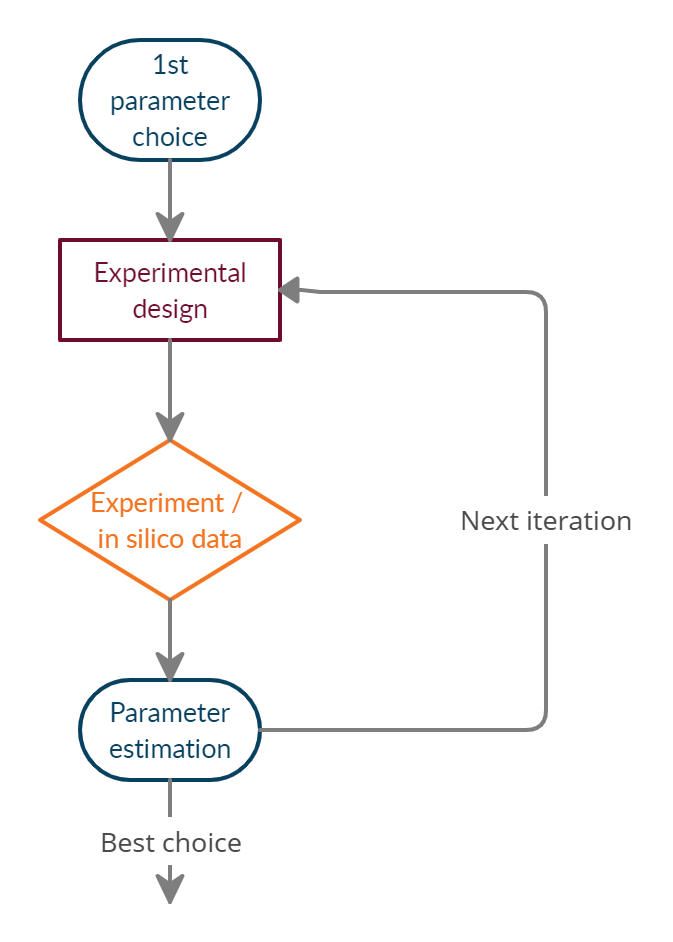
\includegraphics[scale=0.3]{Figures/scheme.png}
    \caption{The iterative process of model optimization for parameter estimation.}
    \label{fig:expdesign_scheme}
\end{figure}
First of all, based on the literature review or some prior data from pilot experiments  the first parameter estimation of the chosen model structure should be done.
The obtained values than can be applied to propose the first optimal experimental design accounting different constraints, e.g., the lab limitations, human resources and etc. 
Depending on availability, either real or numerical experiment should be conducted based on this design to gather measurement or in-silico data. 
This new data can be the used for the new parameter estimations values with corresponding errors.
Here, basically, the first iteration ends. 
After this, using new parameter values, the process can be repeated several times to increase the precision of the parameter estimates till the desired accuracy is achieved.







%
%
%
% ########################################################################
% ########################################################################
\section*{Materials and Methods}
%
%
% ########################################################################
\subsection*{Model Formulation}
\subsubsection*{Theory}
\begin{enumerate}
    \item Define ODE, Jacobian
    \item Which parameters are present?
    \item Differnce between Q-Values, P-Values, Const
\end{enumerate}
\subsubsection*{Code}
\begin{enumerate}
    \item Write ODE, Jacobian functions in python with Q, P, Const\\
    \mintinline[bgcolor=white,style=emacs]{python}{def ode_func(y, t, Q, P, Const):}\\
    \mintinline[bgcolor=white,style=emacs]{python}{def jacobian(y, t, Q, P, Const):}
    \item Define initial values \mintinline[bgcolor=white,style=emacs]{python}{(y0, t0)}
\end{enumerate}
%
% ########################################################################
\subsection*{Parameter Estimation}
\subsubsection*{Theory}
\begin{enumerate}
    \item Log-Likelihood Function
    \item Maximum-Likelihood Estimators
    \item Likelihood Function for Gaussian Noise
\end{enumerate}
\subsubsection*{Code}
\begin{enumerate}
    \item \mintinline[bgcolor=white,style=emacs]{python}{def likelihood_function(fitted_parameter, measurement_data)}
    \item \mintinline[bgcolor=white,style=emacs]{python}{scipy.optimize.minimize}
\end{enumerate}
%
% ########################################################################
\subsection*{Experimental Design}
\subsubsection*{Theory}
\begin{enumerate}
    \item Fischer, Sensitivity Matrix
    \item Observables: Determinant, Eigenvalues, etc.
\end{enumerate}
\subsubsection*{Code}
\begin{enumerate}
    \item How does the user calculate the Fischer Observable?
    \begin{minted}{python}
        def calculate_Fischer_observable(
            parameter_combinations,
            sensitivity_ode_function,
            y0_t0,
            jacobi,
            observable):
    \end{minted}
    \item How do we optimize for best results?
    \begin{minted}{python}
        def optimize_parameters(
            parameter_combinations,
            observable):
    \end{minted}
\end{enumerate}
%
%
%
% ########################################################################
% ########################################################################
\section*{Conclusion}
\begin{enumerate}
    \item Plots: Optimized time points
    \item Observable vs number of measurements
    \item Performance (scaling, limitations, etc.)
    \item 
\end{enumerate}
%
%
%
% ########################################################################
% ########################################################################
\section*{Supporting information}
%
%
%
\nolinenumbers
% ########################################################################
% ########################################################################
\bibliography{predictive-microbiology-software}

\end{document}
%%